\section{Pure Shift \acs{NMR}}
In this section, a survey of some of the most prominent procedures for
producing pure shift spectra is presented.
\subsection{The \acs{2DJ} Experiment}
The \ac{2DJ} experiment~\cite{Aue1976, Morris2009} provided the first means to
achieve broadband homodecoupling. It has the following simple pulse sequence:
\[
    \ang{90} \rightarrow \nicefrac{\tone}{2} \rightarrow \ang{180} \rightarrow \nicefrac{\tone}{2} \rightarrow \ttwo.
\]
After excitation of magnetisation onto the transverse plane, the
indirect-dimension evolution consists of a spin echo, with acquisition
following
immediately afterwards. The result is an \ac{FID} in which only scalar
couplings evolve in $\tone$, as the chemical shifts are refocussed by the
spin echo, while both chemical shifts and scalar
couplings evolve during $\ttwo$. \Iac{FID} generated by the \ac{2DJ}
experiment is hypercomplex, taking the form of \cref{eq:general-fid} with
$D=2$ and $\zeta^{(1)} = \exp(\iu\cdot)$, i.e.
\begin{equation}%
    \begin{split}%
        y_{\none,\ntwo} =
        &\sum_{m=1}^{M} a_m \exp(\iu \phi_m)
            \exp\left(\left(2 \pi \iu \fonem - \etaonem\right) \none \Dtone\right) \times \\
        &\exp\left(\left(2 \pi \iu  \left(\ftwom - \foff\right)
            - \etatwom\right) \ntwo \Dttwo\right)
            + w_{\none,\ntwo}.
    \end{split}%
    \label{eq:jres-fid}%
\end{equation}%
The transmitter offset term has been neglected in the indirect dimension, since
chemical shift evolution does not occur.
For each signal in the \ac{FID}, the indirect- and direct-dimension
frequencies are intimately linked. Consider a \ac{2DJ} dataset generated from a
spin system with $S$ distinct spins.
Under the assumption of the
weak coupling approximation (recall \cref{fn:weak-coupling},
    \cpageref{fn:weak-coupling})
the signals which arise
from a particular spin $s \in \lbrace 1, \cdots, S \rbrace$ form a grouping $G_s
\subset \lbrace 1, \cdots, M \rbrace$ (note that $M \equiv \sum_{s=1}^S \lvert
G_s \rvert$).
All the signals in $G_s$ will have frequencies given by
\begin{subequations}
    \begin{gather}
        \fonem = d_m,\\
        \ftwom = f_{0,s} + d_m,\\
        \forall m \in G_s\notag,
    \end{gather}%
    \label{eq:f1-f2-2dj}%
\end{subequations}
where $f_{0,s}$ is the Larmor frequency of
the spin, and $d_m$ is the displacement
of the signal from $f_{0,s}$, as a result of J-couplings\footnote{
    $d_m$ will be a linear combination of all the J-couplings
    associated with the spin, with all the coefficients being $\pm
    \nicefrac{1}{2}$.
}. Due to this relationship, all peaks in the Fourier domain which are part of
the same multiplet will lie along a line which makes \ang{45} angles to both
the $\Fone$ and $\Ftwo$ axes, as depicted in \cref{fig:jres-spectrum}.a.

One limitation of the \ac{2DJ} experiment is the fact that peaks comprising
pure absorption Lorentzian character cannot be produced. This is since, due
to the absence of a mixing period, it is not possible to acquire a
complementary pair of phase-modulated \acp{FID}; such a pair could be processed
so as to nullify the dispersive contributions (see \cref{subsec:multidim}).
The FT of a \ac{2DJ} \ac{FID} produces a spectrum with phase-twist
peaks; an example is provided in \cref{fig:jres-spectrum}.a. As with
other experiments which produce hypercomplex signals, such as \ac{COSY}, the
data is conventionally displayed in \emph{magnitude-mode}
(\cref{fig:jres-spectrum}.b) in which the absolute value of each complex point
in the spectrum is plotted.

\correction{
When present, another disadvantageous trait of \ac{2DJ} datasets are \emph{strong
coupling artefacts}, which arise due to coherence transfers induced by
the \ang{180} pulse~\cite{Wider1983,Thrippleton2005}.
These are not strictly artefacts, but rather genuine signals which are expected
to be present in the \ac{2DJ} dataset; despite this, the term is widespread in
the literature.
An illustration of the influence of strong coupling effects is provided for an
AB spin system in \cref{fig:jres-ab}. A rigorous description of
the theory behind a \ac{2DJ} experiment for this system is given
in~\cite{Thrippleton2005}.
As well as four \emph{first-order} signals (those that are accounted for
when the weak coupling approximation is invoked)
four additional signals appear in the dataset due to strong coupling effects.
The frequencies and relative amplitudes of the eight signals are stated in
\cref{fig:jres-ab}.a.
}\label{corr:strong-coupling-artefacts}
% \begin{longtable}{c c c}
%     \hline
%     $a$ & $\fone$ & $\ftwo$\\
%     \hline
%     \multicolumn{3}{c}{\textbf{First order signals}}\\
%     \hline
%     1 & $\frac{J_{\text{AB}}}{2}$ & $f_{\text{A}} + \frac{J_{\text{AB}}}{2}$\\
%     1 & $-\frac{J_{\text{AB}}}{2}$ & $f_{\text{A}} - \frac{J_{\text{AB}}}{2}$\\
%     1 & $\frac{J_{\text{AB}}}{2}$ & $f_{\text{B}} + \frac{J_{\text{AB}}}{2}$\\
%     1 & $-\frac{J_{\text{AB}}}{2}$ & $f_{\text{B}} - \frac{J_{\text{AB}}}{2}$\\
%     \hline
%     \multicolumn{3}{c}{\textbf{Strong coupling artefacts}}\\
%     \hline
%     $\rho_{\text{AB}}$ & $\frac{J_{\text{AB}}}{2} + \xi_{\text{AB}}$ & $f_{\text{A}} + \frac{J_{\text{AB}}}{2}$\\
%     $\rho_{\text{AB}}$ & $-\frac{J_{\text{AB}}}{2} + \xi_{\text{AB}}$ & $f_{\text{A}} - \frac{J_{\text{AB}}}{2}$\\
%     $\rho_{\text{AB}}$ & $\frac{J_{\text{AB}}}{2} - \xi_{\text{AB}}$ & $f_{\text{B}} + \frac{J_{\text{AB}}}{2}$\\
%     $\rho_{\text{AB}}$ & $-\frac{J_{\text{AB}}}{2} - \xi_{\text{AB}}$ & $f_{\text{B}} - \frac{J_{\text{AB}}}{2}$\\
%     \hline
%     \caption[
%         The frequencies and relative amplitudes of signals which feature in the
%         \acs{2DJ} spectrum of an AB spin system.
%     ]{
%         The frequencies and relative amplitudes of signals which feature in the
%         \acs{2DJ} spectrum of an AB spin system. The quantities $\xi_{\text{AB}}$
%         and  $\rho_{\text{AB}}$ are defined in \cref{eq:ab-sep,eq:ab-amp},
%         respectively.
%     }\label{tab:jres-ab}
% \end{longtable}
\correction{
Each of the strong coupling artefacts has a direct-dimension frequency that
matches that of one of the
first-order signals. However, each of these signal pairs have indirect
dimension frequencies which differ by $\xi_{\text{AB}}$:
\begin{equation}
    \xi_{\text{AB}} = \frac{1}{2} \sqrt{(f_{\text{A}} - f_{\text{B}})^2 +
    J_{\text{AB}}^2}.\label{eq:ab-sep}
\end{equation}
The magnitude of the displacement is such that strong coupling artefacts are
frequently aliased in the indirect dimension, which tends to have a small
spectral width ($\approx \qty{50}{\hertz}$).
Due to their displacement in the indirect dimension, strong coupling artefacts
lie along different \ang{45} cross sections to the first-order signals
they are associated with.
The intensities of the strong coupling artefacts relative to the
first-order signals is given by:
\begin{equation}
    \rho_{\text{AB}} = \tan^{-1}\left(\frac{J_{\text{AB}}}{f_{\text{A}} - f_{\text{B}}}\right).
    \label{eq:ab-amp}
\end{equation}
From this expression, it can be seen that as the difference in chemical shift
increases, the magnitude of the strong coupling artefacts diminishes; eventually
the weak coupling regime is reached and strong coupling artefacts have a
negligible influence on the data.
}

\begin{figure}%
    \centering%
    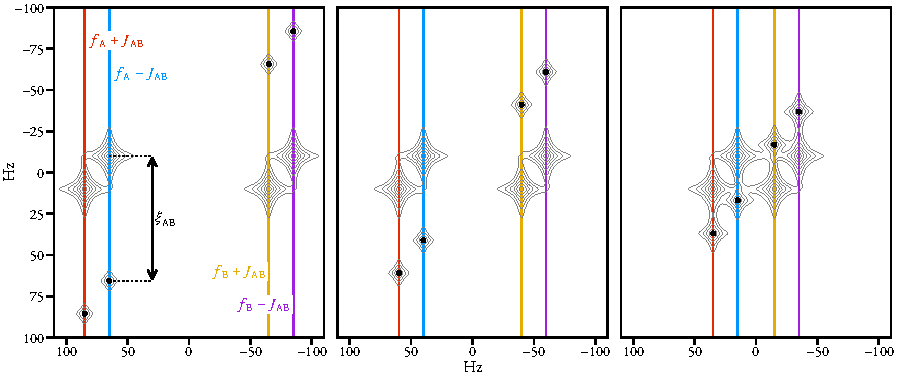
\includegraphics{figures/jres_ab/jres_ab.pdf}
    \caption[
        An illustration of the appearance of \acs{2DJ} spectra for a strongly
        coupled two spin system.
    ]{
        \correction{
            An illustration of the appearance of \acs{2DJ} spectra for a strongly
            coupled AB spin system.
            \textbf{a.} A table of the frequencies and relative amplitudes of
            signals which feature in the \acs{2DJ} dataset of such a
            system. The quantities $\xi_{\text{AB}}$ and  $\rho_{\text{AB}}$
            are defined in \cref{eq:ab-sep,eq:ab-amp}, respectively.
            \textbf{b.} Two examples of magnitude-mode \ac{2DJ} spectra,
            generated using the following spin system specifications:
            \textbf{b1.}
            $f_{\text{A}} = \qty{75}{\hertz}$,
            $f_{\text{B}} = \qty{-75}{\hertz}$,
            $J_{\text{AB}} = \qty{20}{\hertz}$;
            \textbf{b2.}
            $f_{\text{A}} = \qty{25}{\hertz}$,
            $f_{\text{B}} = \qty{-25}{\hertz}$,
            $J_{\text{AB}} = \qty{20}{\hertz}$.
        Along with the 4 first-order
        signals (labelled ``f\hspace{1pt}''), 4 strong coupling artefacts are present in
        each spectrum (labelled ``s''). The artefacts
        have the following amplitudes relative to the first order signals:
        0.133 (b1), 0.381 (b2). Each artefact has a
        direct-dimension frequency which matches that of one of the first-order
        signals; in the indirect dimension the frequencies of each signal pair
        differ by the quantity
        $\xi_{\text{AB}}$, which is:
        \qty{75.7}{\hertz} (b1),
        \qty{26.9}{\hertz} (b2).
        N.B. the spectral width in the indirect dimension (\qty{200}{\hertz}) is
        considerably larger than typical values used for \ch{^1H}
        \acs{2DJ} experiments; this as been done to ensure the strong coupling
        artefacts are not aliased which occurs often in real datasets.
    }
    }
    \label{fig:jres-ab}
    \vspace{20pt}
    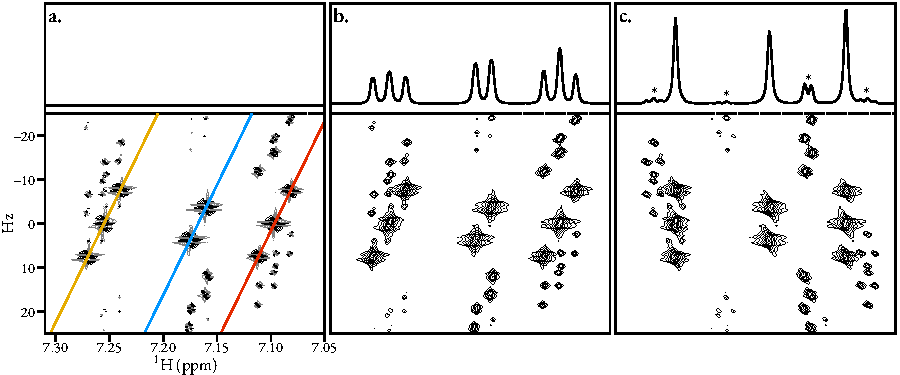
\includegraphics{jres_spectrum/jres_spectrum_new.pdf}%
    \caption[
        A region of a \acs{2DJ} spectrum of strychnine, processed in different
        ways.
    ]
    {%
        A region of a simulated \acs{2DJ} spectrum of strychnine.
        Each panel depicts the spectrum following different processing
        procedures. Below: contour plots of the spectrum.
        Black contours have positive values; grey contours have negative
        values.
        Above: the projection of the spectrum onto the direct dimension ($\Ftwo$).
        \textbf{a.} Spectrum produced by applying sine-bell apodisation
        followed by \ac{FT} in both dimensions.
        Coloured lines denote \ang{45} cross-sections along which first-order
        multiplet structures lie.
        Prominent strong coupling artefacts have been annotated with dotted
        ellipses.
        \textbf{b.} Magnitude-mode spectrum.
        \textbf{c.} Spectrum generated after application of a \ang{45} shear on
        the magnitude-mode spectrum. Peaks marked with an asterisk originate
        from strong coupling artefacts in the \ac{2DJ} spectrum.
   }%
    \label{fig:jres-spectrum}%
    \end{figure}

\subsubsection{The Shear and Projection Approach}
A pure shift spectrum can be acquired from a \ac{2DJ} spectrum by performing a
\ang{45} shear on the spectrum array; each direct-dimension vector in the
spectrum is subjected to a right circular rotation according to
\begin{subequations}
    \begin{gather}
        s_{\none,\ntwo}^{\text{shear}} =
            s_{\none,n^{(2)\prime}}^{\vphantom{{\text{tilt}}}},\\
        n^{(2)\prime} = \left(\ntwo + \left\lfloor
                \frac
                    {\fswone \Ntwo\vpsub{\mathrm{sw}}}
                    {\fswtwo \None\vpsub{\mathrm{sw}}}
                \left(
                    \frac{\None\vpsub{\mathrm{sw}}}{2} - \none
                \right)
            \right\rceil
        \right) \bmod \Ntwo.
    \end{gather}
\end{subequations}
In the limit of continuous sampling, this achieves the relationship
\[
    s^{\text{shear}}\left(\Fone,\Ftwo\right) \equiv s(\Fone, \Ftwo - \Fone).
\]
By performing a \ang{45} shear, chemical shifts and scalar couplings are
separated onto orthogonal axes,
such that the peaks of the sheared spectrum which arise from a given spin all
reside at the same value of $\Ftwo$ (\cref{fig:jres-spectrum}.c). The
effectiveness of the shear is maximised when both $\nicefrac{\fswtwo}{\fswone}$
and $\nicefrac{\Ntwo}{\None}$ are powers of 2. After shearing, projecting the
spectrum onto $\Ftwo$ (i.e. summing along the indirect dimension) leads
to the \ac{1D} pure shift spectrum.
If the spectrum wasn't converted to magnitude-mode prior to shearing and
projecting, the absorptive and dispersive components of the spectrum would
cancel each other out, such that a vector devoid of any signal would be
obtained (\cref{fig:jres-spectrum}.a).
With a magnitude-mode spectrum, the process leads to undesirable pure shift
spectra with broad ``wings'' on account of the presence of dispersive
character, as well as non-linearities. These effects can be suppressed by
appropriate
processing to make the FID envelope symmetric in both dimensions;
sine-bell apodisation and pseudo-echo reshaping~\cite{Bax1981} are common methods.
However, these both cause a significant reduction in sensitivity being
incurred, along with distortions in relative peak amplitudes such that the data
are rendered unsuitable for quantitative applications. Examples of experimental
pure shift spectra produced via sine-bell apodisation can be found in Figures
\ref{fig:quinine-cupid}.a and \ref{fig:camphor-cupid}.a, where severe
discrepancies in peak integrals exist.

\correction{
    When strong coupling artefacts feature in the \ac{2DJ} data,
    spectra produced by shearing and projecting onto $\Ftwo$ will feature
    additional low-intensity nuisance signals\,---\,recall from above that
    these tend to lie along different \ang{45} cross-sections to first-order
    signals in the \ac{2DJ} spectrum\,---\,that compound the task of
    interpreting the spectrum (see peaks marked with asterisks in Figures
\ref{fig:jres-spectrum}.c, \ref{fig:quinine-cupid}.a, and
\ref{fig:camphor-cupid}.a.
}

\subsubsection{Pure Shift Spectra from 2DJ Estimation}
Beyond the shearing and projection method, procedures based on the estimation
of \ac{2DJ} datasets have also been developed to achieve broadband
homodecoupling. Nuzillard introduced
\ac{ALPESTRE}~\cite{Nuzillard1996,Martinez2012}, in which the parameters of each
indirect-dimension FID are estimated using \ac{LPSVD}, such that a set of
parameters $\symbf{\Theta} \in \mathbb{R}^{\Ntwo \times 4M}$ is generated:
\begin{equation}
    \symbf{\theta}_{\ntwo} =
    \begin{bmatrix}
        \bda_{\ntwo}\T &
        \bdphi_{\ntwo}\T &
        \bdf_{\ntwo}\T &
        \bdeta_{\ntwo}\T
    \end{bmatrix}\T.
\end{equation}
The parameters generated are used to propagate each FID backward into
$-\tone$, producing a ``full-echo'':
\begin{equation}
    \begin{split}
        y^{\text{full}}_{\none,\ntwo} = \sum_{m=1}^{M}
            a_{\ntwo,m}
            \exp\left(\iu \phi_{\ntwo,m}\right)
            \exp\left(\left(2 \pi \iu f_{\ntwo,m} \none
            -\eta_{\ntwo,m}  \left\lvert \none \right\rvert \right)\Dtone\right), \\
        \forall \none \in \lbrace -\None + 1, \cdots, 0, \cdots, \None - 1 \rbrace,\ \forall \ntwo \lbrace 0, \cdots, \Ntwo - 1 \rbrace.
    \end{split}
    \label{eq:full-echo}
\end{equation}
\ac{FT} of \cref{eq:full-echo} generates a spectrum whose real component
comprises absorption
Lorentzian character in both dimensions. This opens up the means of producing
pure-shift spectra from the \ac{2DJ} experiment with sharp lineshapes and
without signal loss. A similar approach proposed by Mutzenhardt \emph{et~al.}
instead constructs full echoes via \ac{LP} of each direct-dimension
\ac{FID}, and generates a full echo by propagating into
$-\ttwo$~\cite{Mutzenhardt1999}. Further to these \ac{LP} based methods,
Mandelshtam and co-workers have also illustrated how the \ac{FDM} can be applied
for parametric estimation, followed by pure shift spectrum
construction~\cite{Mandelshtam1997,Mandelshtam1998}.

\subsection{Chunking Methods}
A popular set of experimental techniques for pure shift \ac{NMR} comprises
\ac{2D} pulse sequences in which a short initial section (chunk) of the
\ac{FID} at each increment is retained~\cite{Adams2014}. The acquired chunks are
subsequently concatenated to yield a \ac{1D} pure shift signal.  All of the
sequences are designed such that they refocus the effects J-couplings at a
certain known point in time;
the time at which refocussing occurs is adjusted by incrementing
the indirect-dimension ($\tone$), so as to acquire
different chunks of the pure shift \ac{FID}. It is impossible to refocus the
couplings associated with all spins in a sample simultaneously. Instead, the
chunking methods operate by ensuring that J-refocussing is achieved for a
subset of the spins (the \emph{active spins}) while the rest (the \emph{passive
spins}) are manipulated to ensure J-refocussing of the active spins occurs;
these do not contribute to the final \ac{FID}.

\begin{figure}
    \centering
    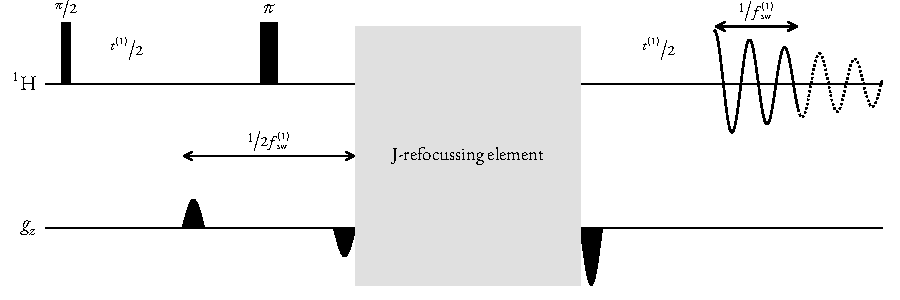
\includegraphics{j_refocussing/j_refocussing.pdf}
    \caption[
        The general form of a pulse sequence used for pure shift \acs{NMR}
        using the chunking approach.
    ]{
        The general form of a pulse sequence used for pure shift \acs{NMR}
        via the chunking approach. Appropriate examples of J-refocussing
        elements include \acs{BIRD}, the \acl{ZS} element, and the
        \acs{PSYCHE} element. The initial chunk of the \ac{FID} (solid
        line) is retained and concatenated with other acquired chunks,
        while the rest (dotted line) is discarded.
    }
    \label{fig:j-refocussing}
\end{figure}
\makeatletter
\AC@reset{BIRD}
\AC@reset{PSYCHE}
\makeatother

A generalised pulse sequence for the chunking approach is depicted in
\cref{fig:j-refocussing}. In the middle of the sequence is a \ang{180} hard
pulse, which inverts all spins. Following this is an element which is designed
to invert the active spins again, while leaving the passive spin coherences
unaffected. As such, the active spins experience no net effect (they
undergo a \ang{360} rotation) while the passive spins experience a net inversion.
This results in the J-couplings associated with the active spins being
refocussed at the point that acquisition starts\footnote{
    In practice, the pulse sequence is usually set up to ensure that the exact
    point of J-refocussing occurs in the middle of each acquired chunk, rather
    that at the start of the chunk. This enables double the amount
    of points to be acquired per increment without noticeable influence from
    J-couplings.
}.
Rather than acquiring a plurality of points, one might envisage that only a
single point should be acquired at each increment to
ensure that the effects of J-couplings are completely negated from the
concatenated signal. However, since the rate of J-coupling evolution is
slow (on the order of \unit{\hertz}), it is far more efficient to acquire a
chunk of points at each iteration for little loss of data quality.

The primary drawback of the chunking approach is that regardless of the
J-refocussing element used, a significant reduction is sensitivity is incurred,
since only a subset of the magnetisation present in the sample contributes to
the detected signal. However, since they are able to produce clean
spectra with absorption lineshapes, these methods have largely superseded the
original \ac{2DJ} shear-and-project approach. A summary of some of the most
prominent J-refocussing elements is now provided.

\subsubsection{\ac{ZS}}
\label{subsec:ZS}
The \ac{ZS} element employs the concept of ``slice-selective excitation'' to
distinguish between active and passive spins~\cite{Zangger1997,Aguilar2010}. It
consists of the simultaneous application of a low \ac{RF} power \ang{180}
pulse\,---\,conventionally, a r-SNOB pulse is used~\cite{Kupce1995}\,---\,and a
weak \ac{PFG} along the laboratory $z$-axis.
The \ac{PFG} induces a change in a given spin's Larmor frequency as a
function of its position in the sample, as was described in
\cref{subsec:diffusion_experiments}. For a low-power \ac{RF} pulse to excite
a given spin, its frequency must be at or very close to its Larmor
frequency.
For spins with different resonance frequencies, the sample region where
excitation occurs differs since their Larmor frequencies must be perturbed by
different extents to match the pulse frequency.
The net effect of the \ac{ZS} element is to invert a particular spin in only a
narrow range of heights in the sample; the spins which are inverted belong to
the pool of active spins, while the remainder are the passive spins.
In order to achieve effective decoupling of a given pair of spins, it is required
that the bandwidth of the selective \ang{180} pulse is smaller than the
difference in their Larmor frequencies. However, with more selective pulses,
a smaller proportion of the spins will be in the active subset, and hence the
\ac{FID}'s sensitivity will be diminished\footnote{
    The sensitivity reduction suffered using the \ac{ZS} element is $\propto
    \nicefrac{\Updelta F}{\gamma g l_z}$, where $\Updelta F$ is the selective
    pulse bandwidth, $g$ is the strength of the \ac{PFG}, and $l_z$ is the
    length of the sample lying within the receiver coil ($\approx
    \qty{1.5}{\centi\meter}$).
}.
Therefore a trade-off exists between effective decoupling of all spins, and
achieving good sensitivity. When strong coupling is present,
the \ac{ZS} element tends to perform poorly relative to other options for this
reason. Keeler and Pell showed that it possible to incorporate the \ac{ZS}
element into the \ac{2DJ} pulse sequence, enabling the generation of \ac{2DJ}
datasets comprising phase-modulated pairs~\cite{Pell2007}. With this approach,
pure shift spectra with far more desirable lineshapes can be generated via the
\ang{45} shear-and-project approach relative to using a magnitude-mode
spectrum.

\subsubsection{Bilinear Rotation Decoupling (BIRD)}
\acused{BIRD}
The \ac{BIRD} element acts to invert spins bound to a low-abundance
heteronuclear isotope, while the remaining spins bound to a high-abundance
isotope are unaffected~\cite{Garbow1982,Bax1983}.
The two most common heteronuclei exploited when using \ac{BIRD} are \ch{^{13}C}
(1.1\% abundance) and \ch{^{15}N} (0.37\% abundance). The loss of sensitivity
is therefore known and constant across samples. In scenarios where strong
coupling exists, \ac{BIRD} can achieve improved sensitivity over \ac{ZS}, due
to the requirement for a highly selective \ang{180} in the \ac{ZS} element as
discussed above.
The \ac{BIRD} method is particularly attractive in scenarios where the
sensitivity penalty due to the involvement of a low-abundance nucleus has
already been paid, for example in sequences where an \ac{INEPT} element is
present~\cite{Paudel2013}. One of \ac{BIRD}'s primary drawbacks is the fact that
geminal protons cannot be decoupled from each other, since such protons are
always in the same active/passive subset. Doublets rather than singlets will
arise in such cases.

\subsubsection{Pure Shift Yielded by Chirp Excitation (PSYCHE)}
\label{subsec:psyche}
\acused{PSYCHE}
The most recent major development in pure shift spectroscopy is the \ac{PSYCHE}
experiment~\cite{Foroozandeh2014,Foroozandeh2018}, which has been hailed for its
ability to generate clean pure shift spectra with better sensitivity relative to
alternative methods. \ac{PSYCHE} is inspired by
the anti z-\ac{COSY} experiment~\cite{Thrippleton2003}, and involves the application
of two low flip-angle ($\beta \ll \ang{90}$) pulses to achieve active/passive
subset creation via coherence selection. The two low flip-angle pulses
are usually either chirp pulses, with the sweep direction of the second being
the opposite of the first, or \emph{saltire} pulses, which are a superposition
of low-to-high and high-to-low chirp pulses. When applied in the presence of a
\ac{PFG}, it has been illustrated that this pair of pulses is very effective at
achieving J-refocussing of the active set of spins, while simultaneously
refocussing other undesired (i.e. non-single quantum) coherences.
The proportions of active and passive spins are dependent on the flip angle of
the chirp pulses; these are $\sin^2 \beta$ and $\cos^2 \beta$,
respectively. With larger flip angles, more signal from unwanted
coherences is present in the final dataset. As with the \ac{ZS} element, this
means there is a compromise that needs to be addressed in order to produce
pure shift spectra that have both acceptable sensitivity and that feature
minimal artefacts; as a rule of thumb, optimal results are typically achieved
when $\beta \approx \ang{20}$.

\correction{
    As was done by Keeler and Pell with the \ac{ZS} element, the \ac{PSYCHE} element
    can be incorporated into \ac{2DJ} experiments to yield \ac{2DJ} spectra
    with absorption-mode lineshapes~\cite{Foroozandeh2015}.
    Furthermore, the \ac{PSYCHE} element can be incorporated as an extra dimension into
    the \ac{2DJ} experiment in order to produce spectra which already feature orthogonal
    separation of the chemical shifts and couplings along the two frequency
    axes~\cite{Kiraly2017}. The \ac{3D} ``\ac{PSYCHE}-\ac{2DJ}'' experiment
    requires long experiment times (typically tens of hours) in order to
    produce a spectrum with well-resolved multiplet structures in the indirect
    dimension.
}\label{corr:PSYCHE-2DJ}
